\documentclass[a4paper, 12pt]{article}
\usepackage{barinov}
\begin{document}
\thispagestyle{empty}
\begin{center}
    \textit{Федеральное государственное автономное образовательное\\ учреждение высшего образования }

    \vspace{0.5ex}

        \textbf{«Московский физико-технический институт\\ (национальный исследовательский университет)»}
\end{center}

\vspace{10ex}

\begin{center}
    \vspace{13ex}

    \so{\textbf{Лабораторная работа №-.-.-}}

    \vspace{1ex}

    по курсу общей физики

    на тему:

    \textbf{\textit{<<>>}}

    \vspace{30ex}

    \begin{flushright}
        \noindent
        \textit{Работу выполнил:}\\  
        \textit{Баринов Леонид \\(группа Б02-827)}
    \end{flushright}
    \vfill
    Долгопрудный \\2019
\newpage
\setcounter{page}{1}
\fancyhead[R]{\nouppercase{\leftmark}}	
\end{center}

\section{Аннотация}
В работе будет измерен показатель преломления воздуха и углекислого
газа с помощью интерферометра Жамена.





\section{Теоретические сведения}
\subsection*{Интерферометры}
Измерительные приборы, использующие явление интерференции, называют
интерферометрами. Оптические интерферометры применяются в физических
экспериментах для измерения длин волн спектральных линий, показателей
преломления прозрачных сред, абсолютных и относительных длин, для
контроля качества оптических деталей и их поверхностей. По числу
интерферирующих пучков интерферометры разделяются на два класса —
многолучевые и двухлучевые. В данном разделе мы рассматриваем
двухлучевую интерференцию. Принцип работы всех двухлучевых
интерферометров одинаков: свет от источника разделяется на два пучка,
идущих по двум различным путям. Затем эти пучки сводятся вместе,
появляющаяся интерференционная картина исследуется с помощью
регистрирующего прибора или визуально.

Вид интерференционной картины зависит от способа получения когерентных
пучков, оптической разности хода, относительной интенсивности,
размеров источника, спектрального состава света. Получают когерентные
пучки двумя способами~--- делением волнового фронта и делением
амплитуды.

В первом способе пучок делится, проходя через два близко расположенных
отверстия (как, например, в опыте Юнга). Метод деления волнового
фронта прост в реализации, его недостаток — большая апертура
интерференции, и как следствие~--- небольшая интенсивность, поскольку
источник должен иметь малые размеры.

Второй способ — деление амплитуды — реализуется, когда пучок делится
на одной или нескольких частично отражающих поверхностей. Деление
амплитуды может применяться при работе с протяжёнными источниками, что
обеспечивает большую интенсивность картины (например, в
интерферометрах Жамена и Майкельсона).


\subsection*{Интерферометр Жамена}

Получить два плеча интерферометра можно делением амплитуды на толстой
плоскопараллельной пластине. Большую разность хода можно
компенсировать использованием второй такой же пластины (рис. 1).
Впервые такую интерференцию наблюдал Брюстер. Эти полосы обычно
называют полосами Брюстера. 


\begin{figure}[H]
    \includegraphics[width=0.7\linewidth]{1} 
    \captionsetup{justification=centering}
    \caption{Схема наблюдения полос Брюстера}
\end{figure}

Пластины располагаются под небольшим углом $\alpha$. Свет от источника
$A$ 
последовательно проходит через две пластины, частично отражаясь.
Интерферируют лучи $E$ и $G$ с минимальной разностью хода, показанные на
рис. 1. Разность хода этих лучей (без учёта разности хода в
воздухе) равна $2nd(\cos\theta_1-\cos\theta_2)$, где $d$ — толщина
пластин, $n$ — их
показатель преломления. Обозначим угол падения луча на первую пластину
$\phi$, тогда на вторую луч падает под углом $\alpha+\phi$. Для малых углов условие
максимума 
\begin{equation}
    2nd(\cos\theta_1-\cos\theta_2) \approx 2dn\left(
        \frac{\phi^2}{2n^2} - \frac{(\phi+\alpha)^2}{2n^2} \right) =
        \frac{2\alpha d}{n}\left(\phi + \frac{\alpha}{2}  \right) =
        m\lambda
        \label{eq:2.68}
\end{equation}

В данном случае мы наблюдаем полосы равного наклона. Из \eqref{eq:2.68}
можно выразить угловое расстояние между полосами:

\[
    \delta \phi = \phi_{m+1} - \phi_m = \frac{\lambda}{2\alpha d}
\]

Подобная схема применяется в интерферометре Жамена, где для исключения
разности хода в воздухе интерферирующие пучки между пластинами идут
перпендикулярно бисекторной плоскости, а сами пластины располагаются
под углом $45^\circ$ к падающему свету (рис. 2). Полосы равного наклона
будут наблюдаться в этом случае как полосы, параллельные ребру
двугранного клина, образованного пластинами (разности хода при
прохождении в воздухе не будет). Присутствие лучей 1 и 4 ухудшает
чёткость интерференционной картины, поэтому их устраняют с помощью
диафрагм.

Так как наблюдаются полосы равного наклона, протяжённый источник
располагают в фокусе коллиматора, а полосы наблюдают в телескоп. Для
идеальных плоскопараллельных пластин в трубе будет видно
геометрическое изображение источника, а на нем будут видны полосы,
ширина которых будет зависеть от угла a между пластинами.

\begin{figure}[H]
    \includegraphics[width=0.9\linewidth]{2} 
    \captionsetup{justification=centering}
    \caption{Ход лучей в интерферометре Жамена}
\end{figure}

При наблюдении в белом свете центральная полоса оказывается
ахроматичной; она окружена двумя глубокими минимумами. Если труба
наблюдения горизонтальна, нулевая полоса оказывается в центре поля
зрения при горизонтальной ориентации клина. При повороте одной из
пластин вокруг горизонтальной оси, параллельной оси клина, изменяется
ширина интерференционных полос, как в рассмотренной системе полос
Брюстера. Если повернуть зеркало вокруг вертикальной оси, меняется
ориентация клина, нулевая полоса смещается вверх или вниз.

Расстояние между двумя плечами интерферометра Жамена будет зависеть от
толщины пластин, и для достаточно толстых пластин в одно из плеч
интерферометра можно поставить кювету с газом, коэффициент преломления
которого можно измерить по смещению интерференционных полос.
Допустимая клиновидность толстых пластин определится дифракционной
расходимостью пучка света в каждом плече. Проверить клиновидность
пластин можно, уменьшив угол между ними а до нуля. Если при этом в
поле зрения будет видно не более двух полос равной толщины, пластины
хорошие. При достаточно толстых пластинах (около 2-3 см) в каждое из
двух плеч интерферометра можно поставить кюветы с газом (как в
интерферометре Релея) для измерения малых изменений коэффициента
преломления газов.



\section{Оборудование}
\textbf{В работе используются:} интерферометр Жамена, газовая кювета,
осветитель, зрительная труба, сильфон, баллон с углекислым газом,
манометр, краны светофильтр.

\subsection*{Экспериментальная установка}
В интерферометре (рис. 3) свет от лампы накаливания Л проходит
коллиматорный объектив, поворотную призму и слегка расходящимся пучком
падает на пластинку $P_1$ под углом $45^\circ$ к ней. Пластины $P_1$ и
$P_2$
закреплены на панели, ниже которой имеются два установочных винта,
позволяющих в небольших пределах поворачивать зеркала. При этом
пластина $P_1$ может поворачиваться вокруг горизонтальной оси (изменение
ширины полос), a пластина $P_2$ — вокруг вертикальной оси (изменение
положения полос).

\begin{wrapfigure}{r}{0.5\linewidth}
    \vspace{-20pt}
    \includegraphics[width=\linewidth]{3}
    \captionsetup{justification=centering}
    \caption{Экспериментальная установка}
\end{wrapfigure}

Между пластинами на пути лучей I и II расположена кювета длины $l$,
состоящая из двух одинаковых камер, закрытых с торцов
плоскопараллельными стеклянными пластинками.

В одну из камер вводится исследуемый газ, а вторая заполнена воздухом
при атмосферном давлении. При этом разность хода $\Delta$, вызванная
разностью показателей преломления газов $\delta n$ приводит к сдвигу
интерференционных полос:
\begin{equation}
    \Delta = \delta n \cdot l
\end{equation}

Сдвиг на одну полосу соответствует дополнительной разности хода
$\Delta = \lambda$.
Определив число полос $m$, на которое сместилась картина, можно
рассчитать
\begin{equation}
    \delta n = \frac{\Delta}{l} = m \frac{\lambda}{l}
\end{equation}

На пути лучей I и II расположен компенсатор Жамена, состоящий из двух
одинаковых плоскопараллельных стеклянных пластинок $J_1$ и $J_2$ (рис.
3).
Если обе пластинки установлены под одинаковым углом к лучам, то и
оптическая длина пути в них для обоих лучей оказывается одинаковой.
Поворот одной из пластинок вокруг горизонтальной оси вызывает
увеличение или уменьшение оптической длины пути соответствующего луча.
Это позволяет скомпенсировать разность хода, возникающую в камерах.
Для точного отсчёта угла поворота одна из пластинок снабжена рычагом,
конец которого смещается при помощи микрометрического винта В.
Пластинки компенсатора ставятся под углом $45^\circ$ к горизонтали, что
позволяет использовать линейную экстраполяцию при измерениях. Смещение
полос можно наблюдать через зрительную трубу Т.

Интерферометр Жамена можно применять для измерения небольших изменений
показателей преломления жидкостей или газов, а также для определения
примесей различных газов в воздухе (например, для измерения
концентрации рудничного газа в шахте).

Показатель преломления n исследуемого газа определяется путём
сравнения с воздухом при атмосферном давлении:

\begin{equation}
    n = n_\text{возд} + \frac{\Delta}{l}
\end{equation}

\subsection*{Газовая система}
Установка, представленная на рис. 4, позволяет заполнять одну камеру
кюветы воздухом при различных давлениях, а вторую — углекислым газом
или воздухом при атмосферном давлении.

Давление воздуха в первой камере изменяется при помощи сильфона С и
измеряется манометром М. Краны K$_1$ и К$_2$ соединяют камеру и манометр с
атмосферой. 


\begin{figure}[H]
    \floatsetup{heightadjust=object,valign=c}
    \begin{floatrow}

        \ffigbox{
        \captionsetup{justification=centering}
        \caption{Газовая система}
    }
        {
        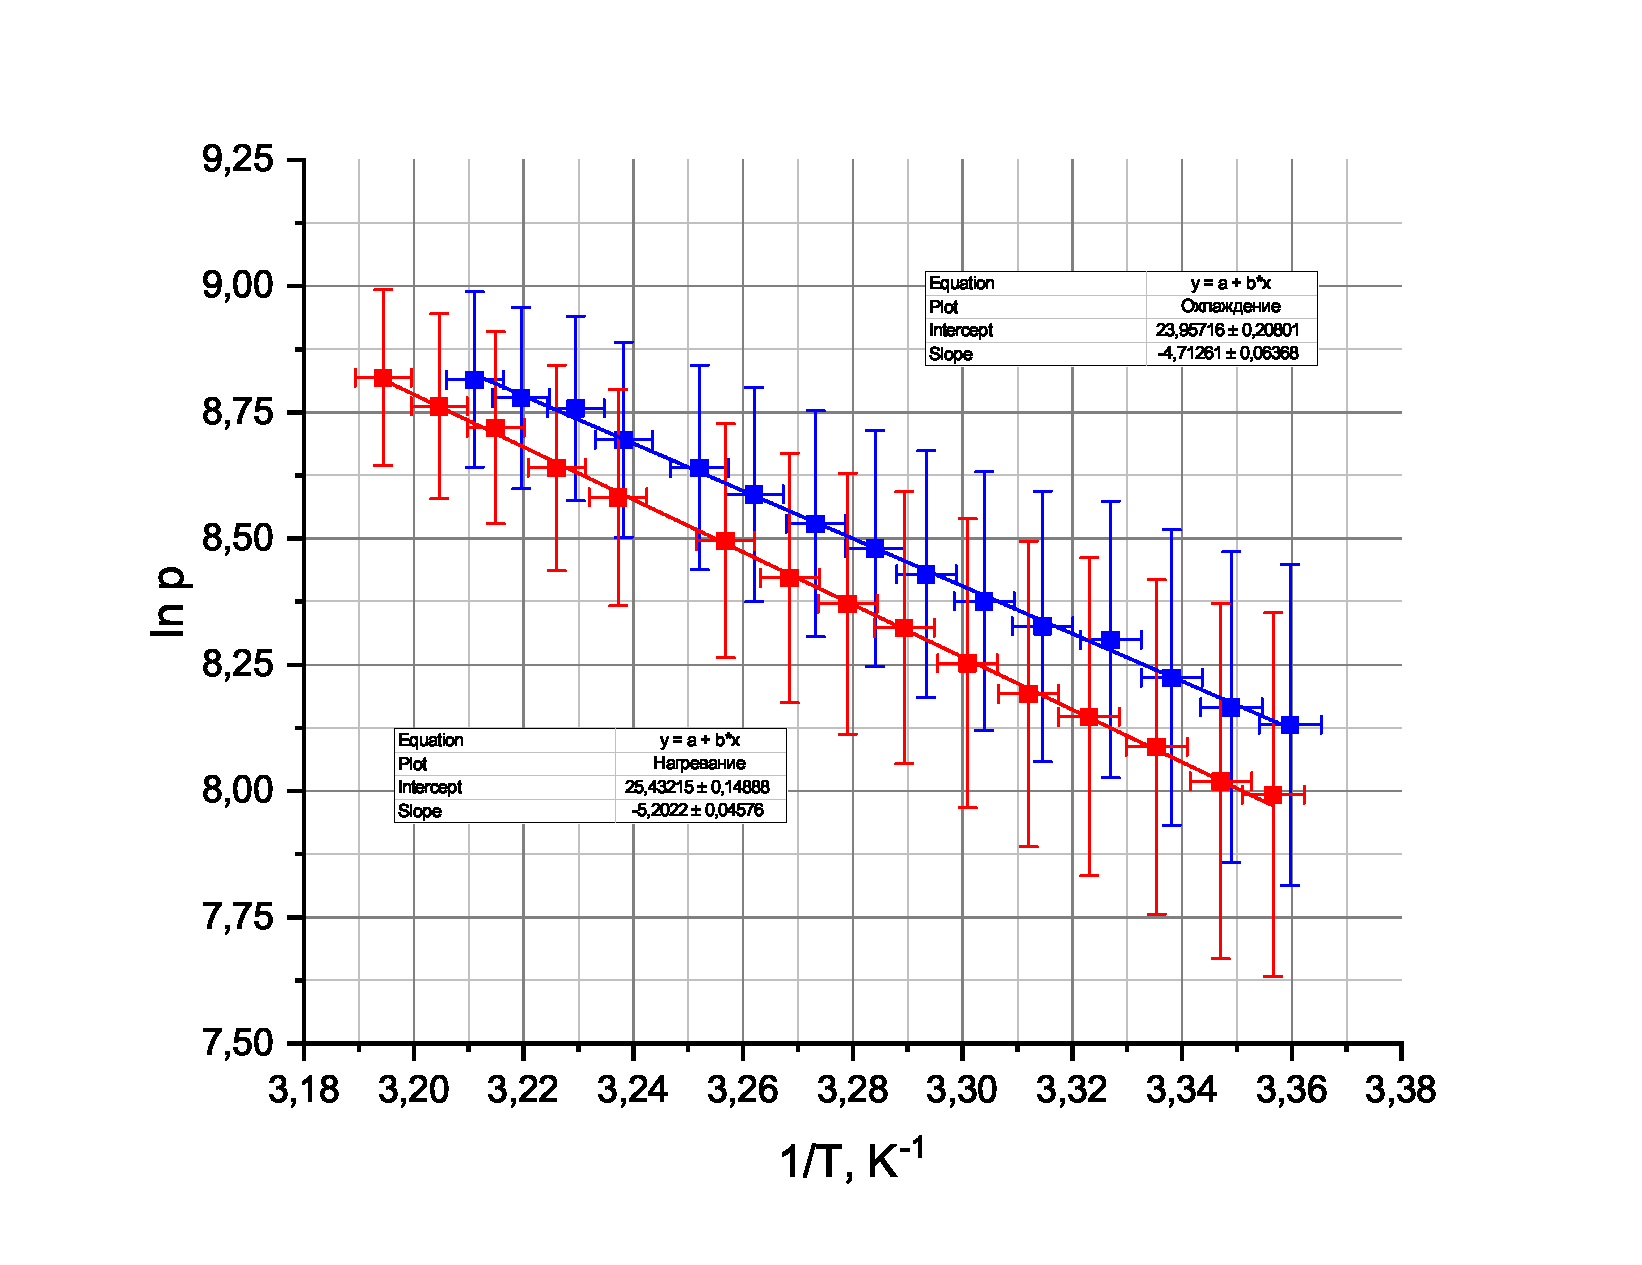
\includegraphics[width=\linewidth]{4}
    }

        \ffigbox{
        \captionsetup{justification=centering}
        \caption{Схема трехходового крана К$_0$}
    }
        {
        \includegraphics[width=0.7\linewidth]{5}
    }
    \end{floatrow}
\end{figure}
Если при атмосферном давлении (открытых кранах K$_1$ и К$_2$) установить
шток сильфона приблизительно в среднее положение, то при закрытом
кране К$_1$ можно, вращая шток, создать в первой камере как повышенное,
так и пониженное давление. Манометр измеряет отклонение давления в
камере от атмосферного в миллиметрах водяного столба.

Для заполнения второй камеры воздухом или углекислым газом при
атмосферном давлении служит трёхходовой кран К$_0$ (рис. 5). В каждом из
трёх рабочих положений этого крана сообщаются два патрубка, соседних с
ручкой крана.

\subsection*{Зависимость показателя преломления газа от давления и
температуры}
Молекулярная оптика устанавливает следующее простое соотношение между
показателем преломления газа и его плотностью:
\begin{equation}
    n = \sqrt{\epsilon} = \sqrt{1+4\pi N \alpha} \approx 1 + 2\pi N
    \alpha
\end{equation}
где $N$ — число молекул в единице объёма, $\alpha$ — поляризуемость молекулы —
коэффициент пропорциональности между дипольным моментом $\vv{p}$ молекулы и
напряжённостью электрического поля $\vv{E}$ ($\vv{p}=\alpha \vv{E}$), $\epsilon$ — диэлектрическая
проницаемость. Принимая во внимание соотношение $P=Nk_\text{Б}T$, где
$P$—
давление в газе, $k_\text{Б}$ — постоянная Больцмана, получим 
\begin{equation}
    n-1 = 2\pi \alpha \frac{P}{k_\text{Б}T}
    \label{eq:6}
\end{equation}

Из 5 следует, что при постоянной температуре изменение показателя
преломления $\Delta n$ пропорционально изменению давления $\Delta P$:
\begin{equation}
    \delta n = \frac{2\pi \alpha}{k_\text{Б}T}\Delta P \quad
    (\text{СГС}) 
\end{equation}
Величина $\delta n$ измеряется с помощью интерферометра Жамена,
$\Delta P$ — с помощью
манометра. Одновременное измерение этих величин (и температуры $T$)
позволяет определить поляризуемость молекул воздуха и, следовательно,
рассчитать по формуле \eqref{eq:6} показатель преломления воздуха для любых
значений $P$ и $T$. Следует отметить, что воздух является смесью
нескольких газов, поэтому под поляризуемостью молекул воздуха нужно
понимать некоторую среднюю величину, определяемую соотношением
\begin{equation}
    \alpha = \frac{1}{N}\sum\limits_i \alpha_i N_i
\end{equation}
где $\alpha_i$ и $N_i$ — поляризуемость и концентрация молекул различных газов,
входящих в состав воздуха, $N$ — общее число молекул в единице объёма.

Формула \eqref{eq:6} позволяет установить связь показателя преломления
газа $n$
при температуре $T$ и давлении $P$ с показателем преломления $n_0$ при
нормальных условиях ($T_0 = 273 \ \text{К}$, $P_0 = 1 \ \text{атм}$):
\begin{equation}
    \frac{n_0-1}{n-1}  = \frac{T}{T_0} \frac{P_0}{P}
\end{equation}


\section{Результаты измерений и обработка результатов}
Длина кюветы $l$, длина волны света, пропускаемого светофильтром
$\lambda$
\[
    l = 10\ \text{см}, \; \lambda = 630-670 \ \text{нм} 
\]

Температура $T$ и давление $p$ в лаборатории:

\[
    T = 297,4\ \text{К}, \; p = 100,1\ \text{кПа}
\]

Прокалибруем компенсатор в единицах $\lambda$, выделив узкий интервал
длин волн с помощью светофильтра.Построим калибровочный график $z_m =
f(m)$ — зависимость отсчёта по
компенсатору от номера совмещённой полосы.


\begin{table}[H]
\centering
\begin{tabular}{|c|c|c|c|c|c|c|c|}
\hline
$m,\ \lambda$ & -4    & -3    & -2   & -1    & 0    & 1    & 2    \\ \hline
$z_m,\ \text{мм}$ & -0,19 & -0,14 & -0,10 & -0,05 & 0,00    & 0,05 &
0,10
\\ \hline \hline  
$m,\ \lambda$ & 3     & 4     & 5    & 6     & 7    & 8    & 9    \\ \hline
$z_m,\ \text{мм}$ & 0,14  & 0,19  & 0,24 & 0,28  & 0,33 & 0,38 & 0,42 \\ \hline
\end{tabular}
\captionsetup{justification=centering}
\caption{Калибровка компенсатора}
\end{table}


\begin{figure}[H]
    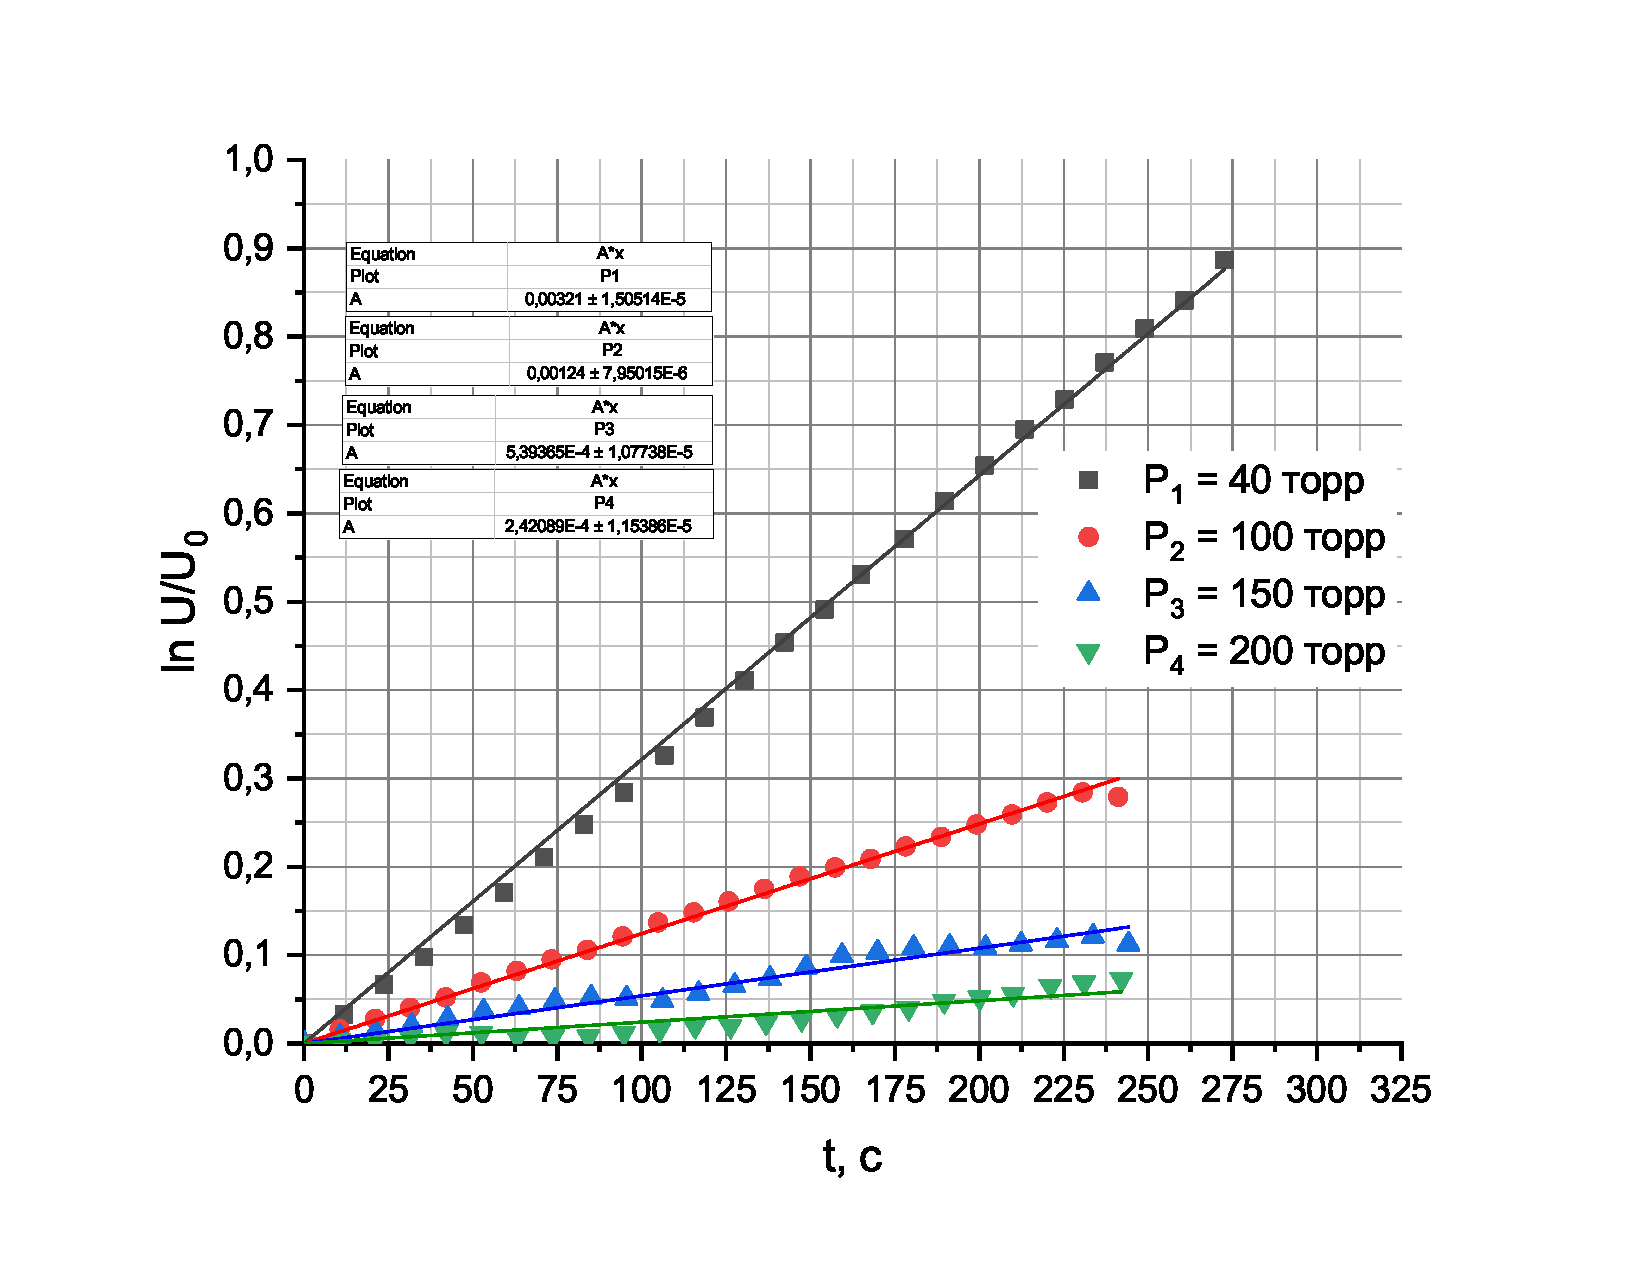
\includegraphics[width=\linewidth]{6} 
    \captionsetup{justification=centering}
    \caption{Калибровка компенсатора}
\end{figure}

Изменяя давление с помощью сильфона и совмещая нулевую полосу
с перекрестием, снимите зависимость показаний компенсатора $z$ открытых
перепада давлений $\Delta P$.

Построим график $z=f(\Delta P)$ (от $+1000$ до $-1000$ мм H$_2$O).
Определим
угол наклона прямой 
\begin{table}[H]
\centering
\begin{tabular}{|c|c|c|c|c|c|c|}
\hline
$\Delta P,\ \text{мм H$_2$O}$ & -600  & -500 & -400  & -300  & -200  & -100  \\ \hline
$z,\ \text{мм}$  & -0,12 & -0,1 & -0,08 & -0,06 & -0,04 & -0,02 \\ \hline
\hline 
$\Delta P,\ \text{мм H$_2$O}$ & 600   & 500  & 400   & 300   & 200   & 100   \\ \hline
 $z,\ \text{мм}$  & 0,12  & 0,1  & 0,08  & 0,06  & 0,04  & 0,02  \\ \hline
\end{tabular}
\captionsetup{justification=centering}
\caption{Зависимость показаний компенсатора $z$ от перепада давления
$\Delta P$}
\end{table}

Коэффициента наклона калибровочного графика (рис. 6):

\begin{equation*}
    \begin{gathered}
        k_1 = z_m/m \\
        k_1 = (47 \pm 2)\ \text{мкм} 
    \end{gathered}
\end{equation*}

Коэффициента наклона графика зависимости показаний компенсатора $z$ от
перепада давления $\Delta P$:

\begin{equation*}
    \begin{gathered}
        k_2 = z/\Delta P\\
        k_2 = (0,200 \pm 0,008)\ \text{мкм/мм H$_2$O}
    \end{gathered}
\end{equation*}

С помощью калибровочного графика и формулы (3)
перейдем от делений компенсатора $\Delta z$ к величине $\delta n$. 

\begin{figure}[H]
    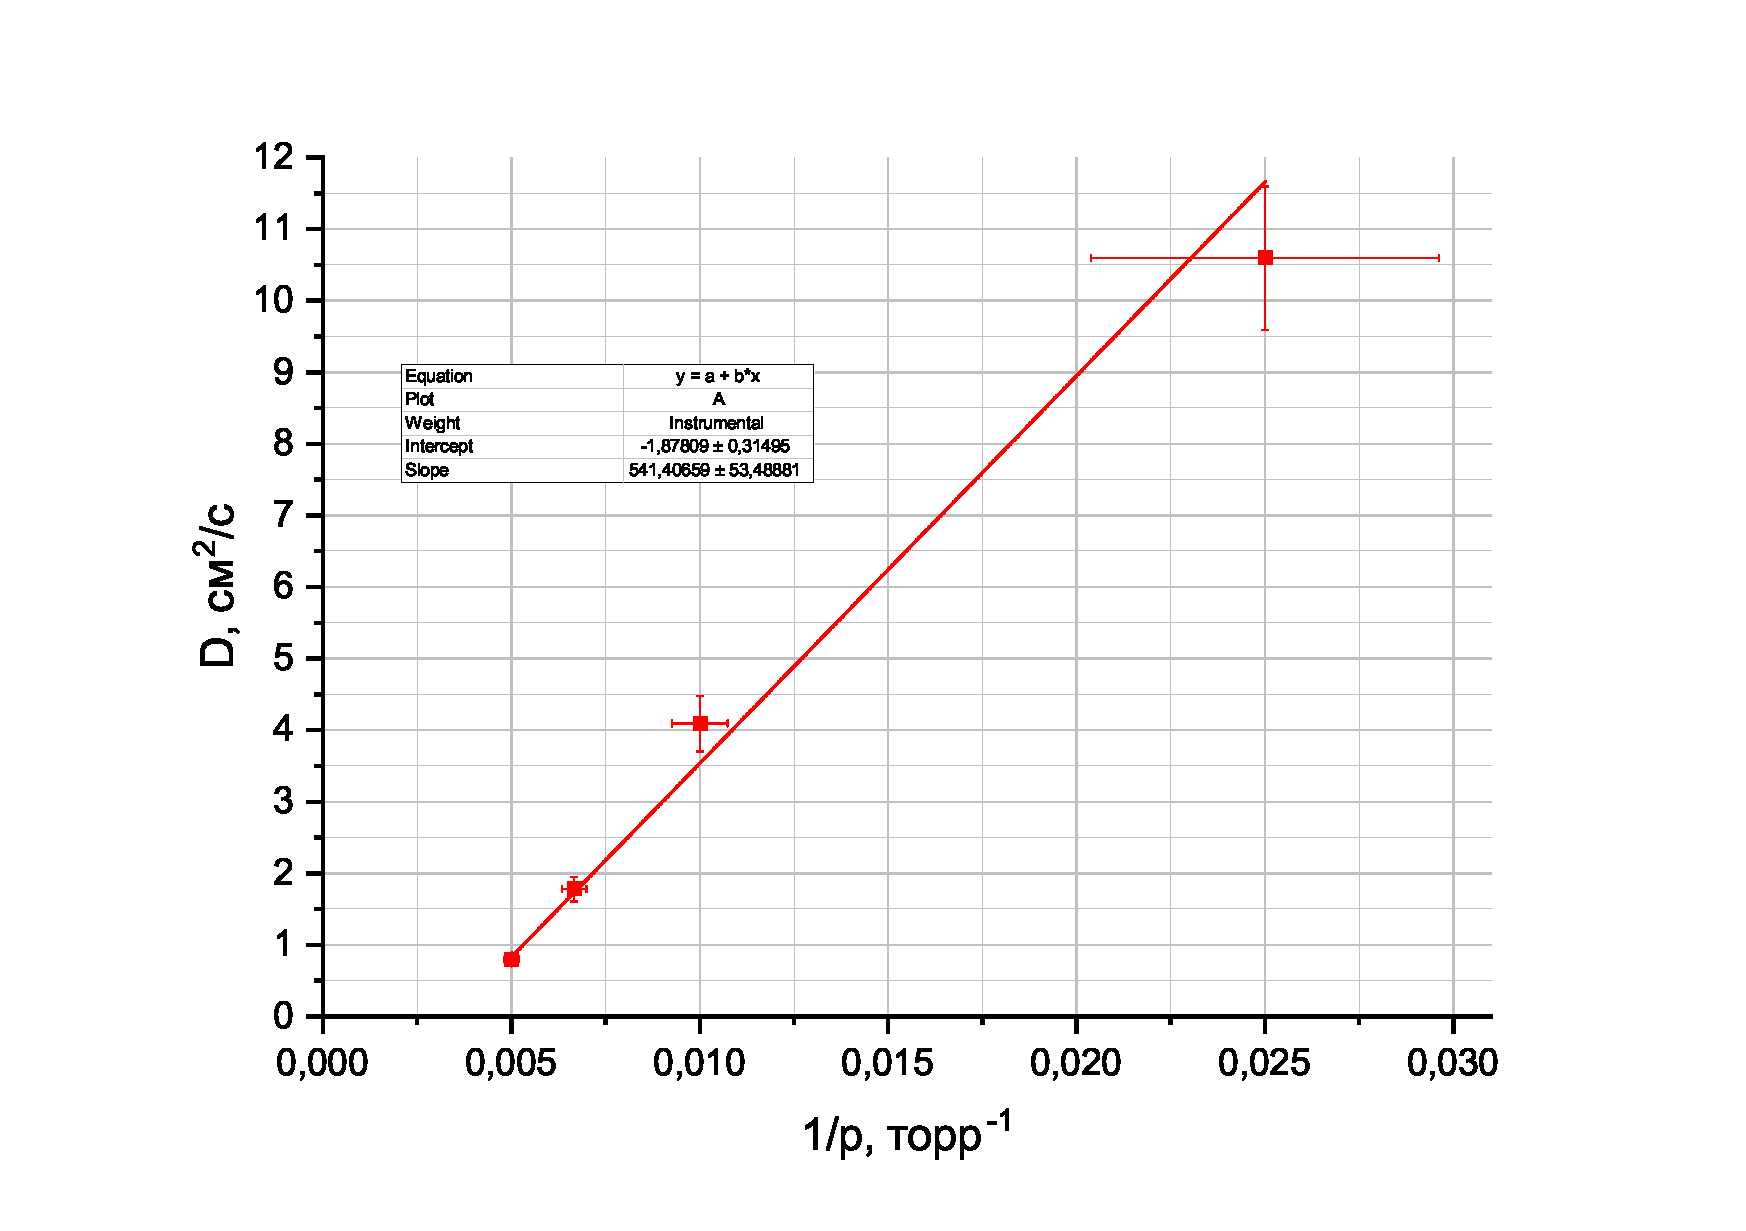
\includegraphics[width=\linewidth]{7} 
    \captionsetup{justification=centering}
    \caption{Зависимость показаний компенсатора $z$ от перепада давлений
    $\Delta P$}
\end{figure}

Из
формул для $k_1$ и $k_2$ видно, что

\[
    m = \frac{k_2}{k_1}\Delta P
\]

Из формулы (3): 

\begin{equation}
    \delta n = \frac{k_2}{k_1}\Delta P \cdot \frac{\lambda}{l}
\end{equation}

Подставляя $\delta n$ из формулы (10) в формулу (6) получим
соотношение из которого выразим поляризуемость молекулы:
\begin{equation}
    \alpha = \frac{k_2}{k_1} \frac{\lambda}{l} \frac{k_\text{Б}T}{2\pi}
\end{equation}

\[
    \alpha = (1,81\pm 0,12)\cdot 10^{-30}\ \text{м}^3, \: \epsilon = 7\%
\]

По формуле (6) рассчитаем показатель преломления воздуха в условиях
опыта:

\[
    n = 1,00027 \pm 0,00002
\]

Пересчитаем показатель преломления воздуха при нормальных условиях
$n_0$ по формуле (9):

\[
    n_0 = 1,00029 \pm 0,00002
\]

Оценим радиус молекулы азота, рассматривая молекулу как металлический
шарик в однородном электрическом поле. В таком случае $\vv{p} = a^3
\vv{E}$, где $a$ --- радиус молекулы. Исходя из того, что $\vv{p} =
\alpha \vv{E}$, получаем, что радиус можно оценить по формуле $a
\approx
\sqrt[3]{\alpha}$:

\[
    a_{N_2} \approx 10^{-10}\ \text{м} 
\]

Рассчитаем показатель преломления $n^{CO_2}$ для углекислого газа в
условиях опыта по формуле (4):

\[
    n^{CO_2} = 1,00053 \pm 0,00008
\]

Пересчитаем показатель преломления углекислого газа $n_{CO_2}^0$ по
формуле (9):

\[
    n_0^{CO_2} = 1,00058 \pm 0,00009
\]

Оценим интервал $\Delta n$, доступный для измерений, исходя из
возможностей компенсатора: минимальная величина $\Delta n$
определяется точностью компенсатора, максимальная --- диапазоном
работы. 
\begin{equation*}
    \begin{gathered}
        \Delta n_{min} = 6\ \text{мкм} \\
        \Delta n_{max} = 25\ \text{см}
    \end{gathered}
\end{equation*}

\section{Обсуждение результатов и выводы}
В работе было исследовано устройство интерферометра Жамена. С помощью
него были измерены показатели преломления воздуха $n$ и углекислого
газа $n^{CO_2}$ в лабораторных условиях. Показатели преломления были
пересчитаны для <<нормальных условий>> $n_0$, $n_0^{CO_2}$
соответственно. Показатель преломления воздуха совпал с теоретическим
значением, однако значение показателя преломления углекислого газа
несколько отличается от теоретического. Это связано с трудностью
определения нулевой полосы после заполнения камеры углекислым газом.
Смещение нулевой полосы составляет $\approx 40$ полос и выходит за
область видимости зрительной трубы. 

\renewcommand{\arraystretch}{1.4}
\begin{table}[H]
\centering
\begin{tabular}{|c|c|c|}
    \hline 
    \makecell[c]{Величина} & \makecell{Экспериментальное \\ значение} &
    \makecell{Теоретическое \\ значение} \\ \hline 
    $n_0$ & $1,00029\pm0,00002$ & $1,000292$ \\ \hline 
    $n_0^{CO_2}$ & $1,00058\pm0,00009$ & $1,000450$ \\ \hline 
\end{tabular}
\captionsetup{justification=centering}
\caption{Сравнение теоретических и экспериментальных значений
показателей преломления воздуха и углекислого газа}
\end{table}






\end{document}
